\documentclass[a4paper, 12pt]{article}

\usepackage{babel}
\usepackage{enumitem}
\usepackage{times}
\usepackage{graphicx}
\usepackage{geometry}
	\geometry{left = 4cm, top = 4cm, right = 3cm, bottom = 3cm}
\usepackage{float}
\usepackage{setspace}
	\setstretch{1.5}
\usepackage{listings}


\begin{document}
\title{\huge\textbf{Tugas Praktikum Pemrograman II (Chapter 3)}}
\date{}

\maketitle


\begin{figure}[!ht]
\begin{center}

\includegraphics[width = 6cm, height = 6cm]{poltekpos.jpg}
\end{center}
\end{figure}

\begin{center}
\vspace{1cm}
Disusun oleh :\\
Dimas Aqila Maulana\\
D4 TI 2C\\
1.18.4.081\\
\vspace{1cm}
\textbf{PROGRAM DIPLOMA IV POLITEKNIK POS INDONESIA} \linebreak
\textbf{POLITEKNIK POS INDONESIA} \linebreak
\textbf{BANDUNG}\linebreak
\textbf{2019}

\end{center}


\thispagestyle{empty}

\chapter{Laporan}
\section{PEMAHAMAN TEORI}
\subsection{FUNGSI}
\begin{enumerate}
	\item Fungsi adalah salah satu blok program yang sudah terorganisir terdiri dari nama fungsi, input variabel dan variabel kembalian. Fungsi digunakan untuk aplikasi anda dan tingkat penggunaan kode yang tinggi agar aplikasi lebih baik.
	\item inputan fungsi digunakan untuk menerima baris input dari user dan mengembalikannya dalam bentuk string.
	\item kembalian fungsi yaitu fungsi akan membaca sebaris input umumnya melalui keyboard sampai nanti dijumpai karakter newline(enter) dan akan mengembalikan string dari inputan tersebut.  
\end{enumerate}
\lstinputlisting[language=Python]{src/KodingTeori1.py}

\subsection{PAKET}
\begin{enumerate}
\item Paket adalah sebuah manifestasi dari konsep namespace hierarkis python.
\item cara pemanggilan paket  
\lstinputlisting[language=Python]{src/KodingTeori2.py}
\end{enumerate}

\subsection{KELAS}
\begin{enumerate}
\item kelas adalah prototipe yang ditentukan oleh pengguna untuk objek yang mendefinisikan seperangkat atribut yang menjadi ciri khas dari sebuah kelas apa pun. Class digunakan untuk membuat kelas baru dan nama kelas diikuti kanca kunci titik dua. 
\item Objek adalah perwujudan dari sebuah class. Bila kelas adalah prototipe nya, dan objek adalah barang jadinya. 
\item atribut yaitu semua class yang membuat objek dan semua objek tersebut mengandung karakteristik.
\item method merupakan fungsi yang didefinisikan di dalam suatu class.
\end{enumerate}
\lstinputlisting[language=Python]{src/KodingTeori3.py}
\subsection{Cara pemanggilan library kelas dari instansiasi dan pemakaiannya contoh dengan program}
untuk membuat objek dari sebuah kelas, kita memanggil nama kelas dengan argumen yang sesuai dengan   fungs pada saat kita mendefinisikannya.
\\cara pemanggilan\\
\lstinputlisting[language=Python]{src/KodingTeori4.py}
\subsection{Pemakaian paket dengan perintah from kalkulator import penambahan}
Pertama-tama kalian harus membuat program kalkulator.py untuk bisa melakukan penambahan sperti di bawah
\lstinputlisting[language=Python]{src/KodingTeori5.py}
\subsection{Pemakaian paket fungsi apabila file library ada di dalam folder}
Untuk pemakaian paket fungsi apabila file library berada di folder yaitu untuk dapat melakukan atau menjalankan kalkulator yang berada di file folder.
\lstinputlisting[language=Python]{src/KodingTeori6.py}
\subsection{Pemakaian paket kelas apabila file library ada di dalam folder}
Untuk pemakaian paket kelas apabila file library berada di folder.Mahasiswa yaitu file Mahasiswa untuk melakukan atau menjalankan kode yang berada di file folder Mahasiswa tersebut.
\lstinputlisting[language=Python]{src/KodingTeori7.py}
\section{KETERAMPILAN PEMROGAMAN}
\lstinputlisting[language=Python]{src/NPM1.py}
\lstinputlisting[language=Python]{src/NPM2.py}
\lstinputlisting[language=Python]{src/NPM3.py}
\lstinputlisting[language=Python]{src/NPM4.py}
\lstinputlisting[language=Python]{src/NPM5.py}
\lstinputlisting[language=Python]{src/NPM6.py}
\lstinputlisting[language=Python]{src/NPM7.py}
\lstinputlisting[language=Python]{src/NPM8.py}
\lstinputlisting[language=Python]{src/NPM9.py}
\lstinputlisting[language=Python]{src/NPM10.py}
\lstinputlisting[language=Python]{src/kalkulator.py}
\lstinputlisting[language=Python]{src/Mahasiswa.py}
\lstinputlisting[language=Python]{src/Ngitung.py}
\lstinputlisting[language=Python]{src/3lib.py}
\lstinputlisting[language=Python]{src/main.py}
\lstinputlisting[language=Python]{src/kelas3lib.py}
\lstinputlisting[language=Python]{src/main.py}
\section{KETERAMPILAN PENANGANAN ERROR}
\lstinputlisting[language=Python]{src/KeterampilanPenangananError.py}
\section{LAMPIRAN PLAGIARISM}
\begin{figure}[H]
		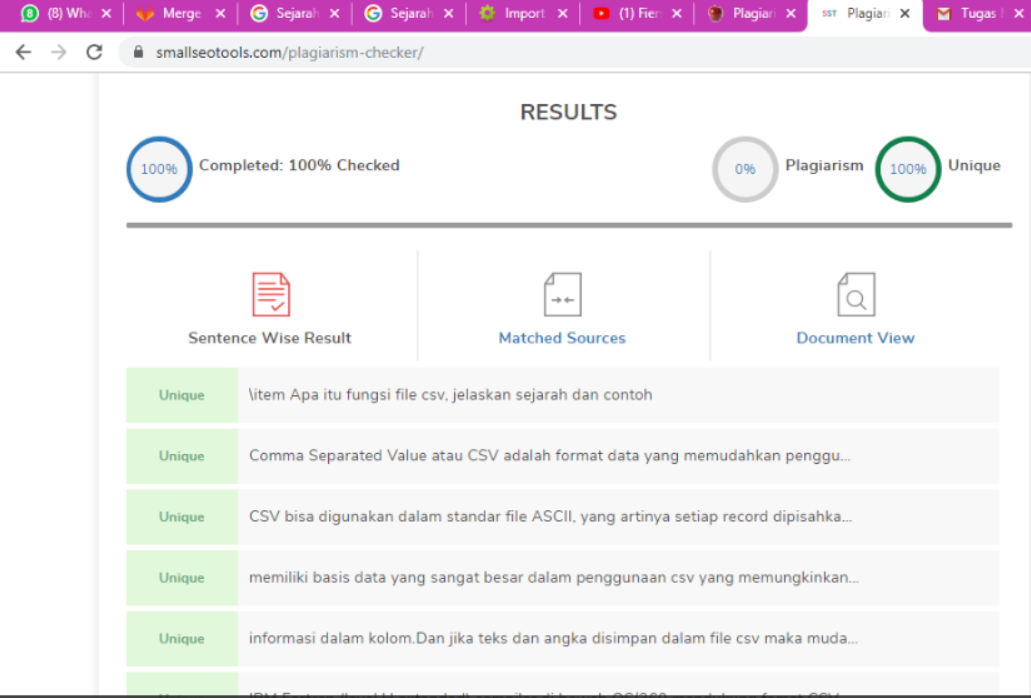
\includegraphics[width=4cm]{figures/1184065/ss1.PNG}
		\centering
		\caption{Screnshoot Plagiarism}
	\end{figure}
	\begin{figure}[H]
		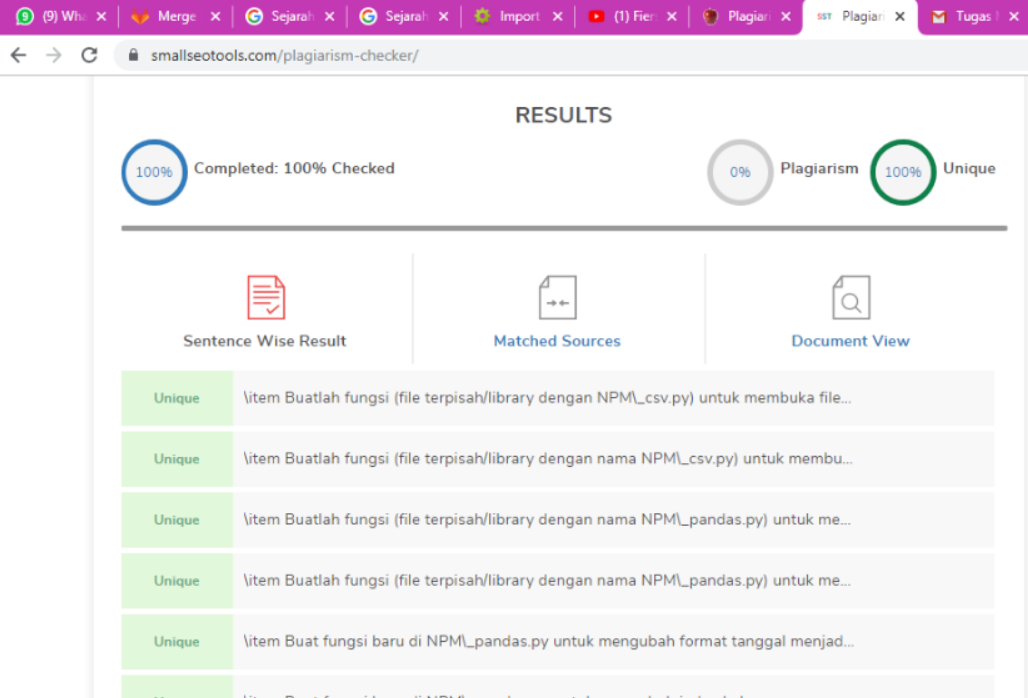
\includegraphics[width=4cm]{figures/1184065/ss2.PNG}
		\centering
		\caption{Screnshoot Plagiarism}
	\end{figure}
\section{LINK YOUTUBE}
\begin{enumerate}
\item \href{https://youtu.be/FDE8KrHC4m4}{klik}
\item \href{https://youtu.be/qzmEN1LVhsM}{klik}
\item \href{https://youtu.be/3UKVrJmwmYo}{klik}
\item \href{https://youtu.be/3UKVrJmwmYo}{klik}
\end{enumerate}








\section{Fungsi}
	\subsection{pemahaman teori}
		\begin{enumerate}
			\item fungsi\\
			Fungsi adalah blok kode yang akan dieksekusi ketika dipanggil dalam sebuah program.\\
			
			\item Parameter\\
			Parameter adalah inputan sebuah fungsi yang bertujuan untuk menyimpan suatu nilai.
			
			\item Return\\
			Return berfungsi untuk mengembalikan suatu nilai yang telah di proses dalam suatu fungsi dan mengakhiri sebuah fungsi.
			\begin{lstlisting}[language=Python]
			def fungsi(x,y):
					z=x+y
					return z
			\end{lstlisting}
			
			\item Item Paket\\
			Item Paket adalah sebuah direktori dengan suatu file python dan file dengan nama \_init\_.py. jadi sebuah direktori yang didalamnya ada sebuah python dengan nama \_init\_.py,dan dianggap sebagai paket oleh python tersebut, untuk memanggil sebuah paket atau library adalah dengan cara menekan \textit{import} nama paket atau library tersebut lalu paket atau library tersebut dapat digunakan.
			\begin{lstlisting}[language=Python]
			from kampus import mahasiswa
			\end{lstlisting}
			
			\item Class\\
			Class adalah sebuah blueprint dari suatu objek yang akan di bangun.
			\begin{lstlisting}[language=Python]
class World:
    def __init__(self,World):
        self.World = World
    def heloWorld(self):
        print("Helo",World)
			\end{lstlisting}
			
			\item Objek memiliki suatu variabel dan kode yang saling terhubung. objek di buat dengan adanaya suatu class.
			\begin{lstlisting}[language=Python]
#import kelas terlebih dahulu
import kelas3lib
#membuat object
cobakelas=kelas3lib.Kelas3ngitung(npm) 
hasilkelas=cobakelas.npm1()
			\end{lstlisting}
			
			\item Attribut\\
			Attribut adalah sebuah tempat tampungan dari sebuah data atau perintah yang berhubungan dengan attribut tersebut.
			\begin{lstlisting}[language=Python]
Class Kelas3ngitung:
	#pendefinisian attribute
    def __init__(self,World):
        self.World = World
			\end{lstlisting}
			
			\item Method\\
			Method adalah sebuah fungsi yang ada didalam suatu class.
			\begin{lstlisting}[language=Python]
class world:
    def __init__(self,world):
        self.world = world
    #Pembuatan method pada class
    def world(self):
       	print("hello",world,",apa kabar ?")
			\end{lstlisting}
			
			\newpage \item Contoh membuat sebuah library, contoh disini kita membuat pada folder library:
			\begin{lstlisting}{language=Python}
def hello():
    print("Hello world")
			\end{lstlisting}

			\item Contoh jika kita ingin memanggil sebuah fungsi dari suatu library pada main program kita harus terlebih dahulu melakukan import:
			\begin{lstlisting}{language=Python}
#import library yang telah dibuat
import library
#pemanggilan fungsi pada library
library.hello()
			\end{lstlisting}
			
			\item Pemakaian package from kalkulator import penambahan
			\begin{lstlisting}{language=Python}
from kalkulator import penambahan
			\end{lstlisting}
kode diatas merupakan perintah program yang memanggil sebuah package terlebih dahulu baru menambahkan source code penambahan, kode diatas dapat dibaca seperti ini "import penambahan dari folder kalkulator"

			\item Pemanggilan library dalam sebuah folder\\
			untuk mengakses sebuah library dalam sebuah folder kita perlu menuliskan foldernya terlebih dahulu, setelah itu kita mengimport nama librarynya, contoh:
			\begin{lstlisting}{language=Python}
from mahasiswa import kampus
			\end{lstlisting}
artinya dalam package mahasiswa akan memakai atau menggunakan suatu library kampus

			\item Pemanggilan class dalam sebuah folder\\
			untuk mengakses sebuah class dalam sebuah folder kita perlu menuliskan foldernya terlebih dahulu lalu kita  mengimport nama class nya, contoh :
			\begin{lstlisting}{language=Python}
from mahasiswa import kampus
			\end{lstlisting}
artinya dalam package mahasiswa akan memakai atau menggunakan suatu class kampus
			
			\end{enumerate}

    \newpage			
	\subsection{Ketrampilan Pemrograman}
			\begin{enumerate}
				\item \lstinputlisting[language=Python]{src/soal1.py}
				\newpage \item \lstinputlisting[language=Python]{src/soal2.py}
				\item \lstinputlisting[language=Python]{src/soal3.py}
				\item \lstinputlisting[language=Python]{src/soal4.py}
				\item \lstinputlisting[language=Python]{src/soal5.py}
				\item \lstinputlisting[language=Python]{src/soal6.py}
				\item \lstinputlisting[language=Python]{src/soal7.py}
				\item \lstinputlisting[language=Python]{src/soal8.py}
				\item \lstinputlisting[language=Python]{src/soal9.py}
				\item \lstinputlisting[language=Python]{src/soal10.py}
				\item \lstinputlisting[language=Python]{src/lib3.py}
				\item \lstinputlisting[language=Python]{src/kelas3lib.py}
				\item \lstinputlisting[language=Python]{src/main.py}
	
\end{enumerate}

\end{document}

